% ═══════════════════════════════════════════════════════════
% §5 Results: Tuning & Optimization
% ═══════════════════════════════════════════════════════════
\section{Results: Tuning \& Optimization}
\label{sec:results-tuning}

\subsection{Hyperparameter Effects (RQ3)}

Section~\ref{sec:results-characterization} established that framework selection contributes only $\sim$5\% throughput variation, while the gap attribution identified autoregressive generation as the dominant efficiency bottleneck. We now demonstrate that hyperparameter choices directly attacking this bottleneck yield far larger effects ($>$30\%). We sweep four knobs on Unsloth BF16 (50 steps each, Table~\ref{tab:sweep}), reporting results ordered by effect magnitude.

\paragraph{Sequence length (+30.8\%).} Reducing max completion from 512 to 256 tokens yields one of the largest single-knob improvements (171.5 vs 131.1 \toksec{}). This directly attacks the attention mechanism's $O(n^2)$ memory access pattern, which is especially costly on RDNA3's 960 GB/s bandwidth. Shorter completions also reduce generation time, shrinking the bandwidth-bound phase identified in \S\ref{sec:gap-attribution}.

\paragraph{Generations G (+31.2\%).} Increasing G from 2 to 8 improves throughput from 124.5 to 163.4 \toksec{}. Higher G generates more tokens per training step, increasing the ratio of compute-bound training operations (27.2\% \mfuprac{}) relative to bandwidth-bound generation (0.23\% \mfuprac{}). The training step's efficiency thus dominates the time-averaged metric when amortized over more generated tokens.

\paragraph{Batch size (+33.4\%).} Moving from b1$\times$4 to b2$\times$4 improves throughput from 97.9 to 130.6 \toksec{}. Larger effective batches produce larger GEMM operations with higher arithmetic intensity, shifting operations from the bandwidth-bound toward the compute-bound regime. The b1$\times$4 configuration's poor performance (1.78\% \mfuprac{}) confirms that insufficient batch size starves the compute units on RDNA3.

\paragraph{Gradient checkpointing (+2.8\%).} Disabling checkpointing yields only 134.8 vs 131.1 \toksec{} (+2.8\%) while consuming 16.5\,GB vs 13.9\,GB VRAM (+18\%). With LoRA's 1.9\% trainable fraction~\citep{hu2022lora}, most activations are frozen and require no gradient storage, making the recompute savings minimal. The poor VRAM-throughput tradeoff confirms that checkpointing should remain enabled.

We note that sweep results use single seeds; however, observed effect sizes ($>$30\%) exceed B1 measurement variance ($\sigma \approx 2\%$) by 15$\times$, making spurious findings highly unlikely.

\subsection{Interaction Effects and Optimal Configuration}

Individual knob effects suggest that combining favorable settings should yield multiplicative gains. The optimal configuration (G=2, b2$\times$4, seq=256, ckpt=on) achieves 178.5 \toksec{} at 3.25\% \mfuprac{} with 12.1\,GB VRAM, representing a 36.2\% throughput improvement over the default (G=4, b1$\times$8, seq=512: 131.1 \toksec{}).

A notable interaction: G=2 outperforms G=4 in the combined configuration (178.5 vs 171.5 \toksec{}), reversing the single-knob trend where higher G is better. This occurs because seq=256 already minimizes generation time per token; at this low generation overhead, the marginal benefit of higher G (amortizing generation) diminishes, while G=2's smaller generation batch leaves more VRAM headroom for the b2$\times$4 training batch to produce larger GEMMs.

Figure~\ref{fig:pareto} maps the VRAM-throughput tradeoff. The Pareto frontier reveals two practical operating points: the throughput-optimal (178.5 \toksec{}, 12.1\,GB) and a VRAM-constrained alternative (171.5 \toksec{}, 12.1\,GB with G=4, b1$\times$8, seq=256) for users requiring lower per-step memory variance.

\subsection{Practical Recommendations}

Based on the preceding analysis, we recommend the following configuration for GRPO post-training of 3B-scale models on consumer RDNA3: G=2, effective batch 2$\times$4, max completion length 256, BF16 precision, gradient checkpointing enabled. This achieves 178.5 \toksec{} at 3.25\% practical MFU within 12.1\,GB VRAM.

The recommendation is workload-conditional: it assumes rule-based rewards with short verifiable completions (e.g., math, code). Tasks requiring longer generations (e.g., open-ended writing) should increase seq\_len to 512 and accept the $\sim$30\% throughput reduction. The dominance of sequence length as an optimization lever (connecting directly to the bandwidth bottleneck identified in \S\ref{sec:gap-attribution}) suggests that any technique reducing effective generation length, including speculative decoding or early stopping, would yield proportional efficiency gains on this architecture.

% ─── Floats集中放置（正文不被截断） ───

% Table 4: Hyperparameter sweep results
% Added ↑ arrows for metric direction, bold optimal
\begin{table}[t]
\centering
\footnotesize
\setlength{\tabcolsep}{3.5pt}
\caption{Hyperparameter sweep results (Unsloth BF16, 50 steps, steady-state corrected caliber). $\uparrow$ indicates higher is better.}
\label{tab:sweep}
\begin{tabular}{@{}lccc@{}}
\toprule
\textbf{Configuration} & \textbf{tok/s} $\uparrow$ & \textbf{\mfuprac} $\uparrow$ & \textbf{VRAM} \\
\midrule
\multicolumn{4}{l}{\textit{Generations (G)}} \\
\quad G=2, b1$\times$8, 512 & 124.5 & 2.27\% & 13.9G \\
\quad G=4, b1$\times$8, 512 & 131.1 & 2.39\% & 13.9G \\
\quad G=8, b1$\times$8, 512 & 163.4 & 2.98\% & 13.9G \\
\midrule
\multicolumn{4}{l}{\textit{Effective Batch Size}} \\
\quad G=4, b1$\times$4, 512 & 97.9 & 1.78\% & 13.8G \\
\quad G=4, b2$\times$4, 512 & 130.6 & 2.38\% & 13.9G \\
\midrule
\multicolumn{4}{l}{\textit{Gradient Checkpointing}} \\
\quad G=4, b1$\times$8, noCkpt & 134.8 & 2.46\% & 16.5G \\
\midrule
\multicolumn{4}{l}{\textit{Sequence Length}} \\
\quad G=4, b1$\times$8, 256 & 171.5 & 3.13\% & 12.1G \\
\quad G=4, b1$\times$8, 1024 & 124.1 & 2.26\% & 13.9G \\
\midrule
\multicolumn{4}{l}{\textit{Combined Optimal}} \\
\quad \textbf{G=2, b2$\times$4, 256} & \textbf{178.5} & \textbf{3.25\%} & \textbf{12.1G} \\
\quad G=2, b1$\times$8, 256 & 172.4 & 3.14\% & 12.1G \\
\bottomrule
\end{tabular}
\end{table}


\begin{figure}[tbp]
\centering
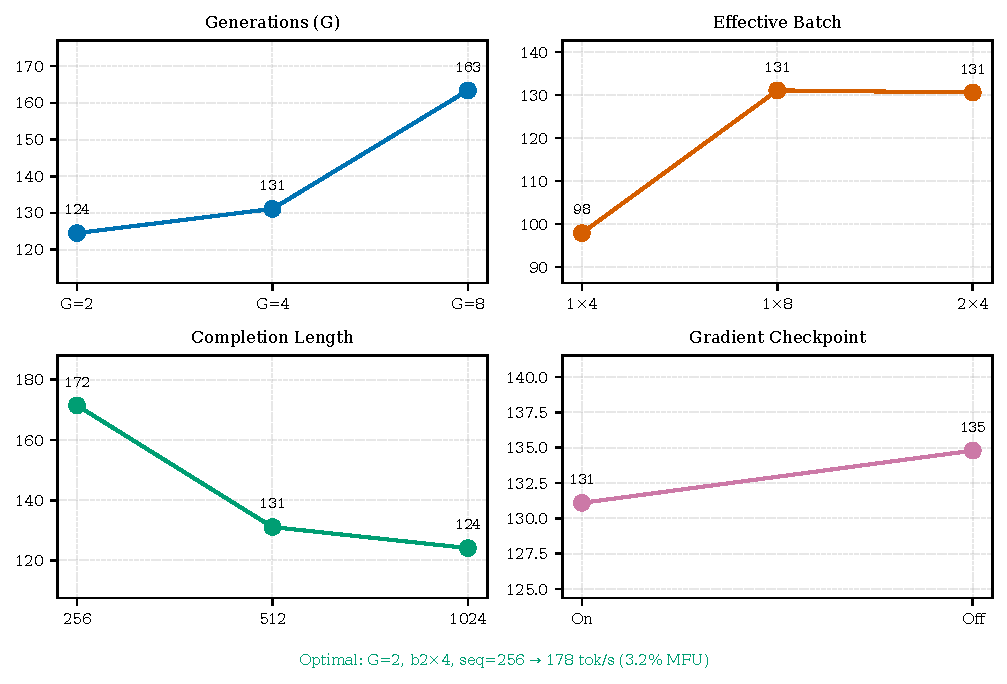
\includegraphics[width=\textwidth]{figures/fig_sweep.pdf}
\caption{Hyperparameter sweep by dimension (baseline: G=4, b1$\times$8, 512).}
\label{fig:sweep}
\end{figure}

\begin{figure}[tbp]
\centering
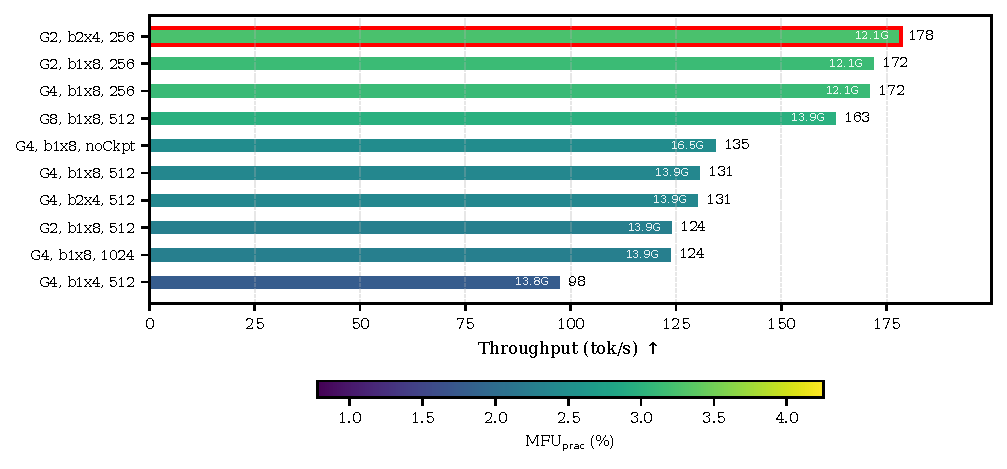
\includegraphics[width=0.85\textwidth]{figures/fig_pareto.pdf}
\caption{Throughput by configuration. Color indicates \mfuprac{}; red border marks optimal.}
\label{fig:pareto}
\end{figure}
